% !TeX program = xelatex
% Q1/Q2 section review only. User-supplied CUMCM template style is unchanged.
\documentclass[zihao=-4,a4paper,UTF8,fontset=none]{ctexart}
\usepackage{cumcm2026}
% Reuse the supplied fonts without duplicating the original template directory.
\newcommand{\TemplateFontPath}{../../downloads/cumcm-latex-template-original-20260911/fonts/}
\setmainfont{TimesNewRoman.ttf}[
 Path=\TemplateFontPath,
 BoldFont=TimesNewRomanBold.ttf,
 ItalicFont=TimesNewRomanItalic.ttf,
 BoldItalicFont=TimesNewRomanBoldItalic.ttf
]
\setCJKmainfont[Path=\TemplateFontPath,BoldFont=SimHei.ttf]{SimSun.ttc}
\setCJKfamilyfont{zhsong}[Path=\TemplateFontPath]{SimSun.ttc}
\setCJKfamilyfont{zhhei}[Path=\TemplateFontPath,BoldFont=SimHei.ttf]{SimHei.ttf}
\setCJKmonofont[Path=\TemplateFontPath,BoldFont=SimHei.ttf]{SimSun.ttc}
\providecommand{\songti}{}
\providecommand{\heiti}{}
\renewcommand{\songti}{\CJKfamily{zhsong}}
\renewcommand{\heiti}{\CJKfamily{zhhei}}
\title{无线电干扰源的快速自动定位与清除：问题一、二章节审阅稿}
\widowpenalty=10000
\clubpenalty=10000
\begin{document}
% This wrapper deliberately contains no full-paper abstract or Q3/Q4 sections.
\begin{center}
 {\heiti\zihao{3} 无线电干扰源的快速自动定位与清除}\par
 \vspace{0.4em}
 {\heiti 问题一、二章节审阅稿}
\end{center}
\section{问题一：有界测向误差下的定位区域与清除判据}
\label{sec:q1}

\subsection{测向误差的集合表示}
设静止干扰源的位置为 $g\in\mathbb R^2$，第 $i$ 个检测点为 $s_i$，获得的示向度为 $\theta_i$。题目给出测向误差处于 $[-1^\circ,1^\circ]$，且同一地点重复检测的误差不变\cite{problem2026}。因此，采用包含所有允许位置的集合表示不确定性，不将重复读数视为独立样本，也不假设误差服从均匀分布或高斯分布。有界误差下用楔形交集描述测向不确定性，与文献\cite{tokekar2013}所研究的几何表示相联系；本文后续结论由本题约束直接推导。

令 $u(\alpha)=(\cos\alpha,\sin\alpha)^{\mathsf T}$，二维叉积记为 $[a,b]=a_xb_y-a_yb_x$，则一次读数对应的闭楔形为
\begin{equation}
 W_i(\delta)=\left\{p:
 [u(\theta_i-\delta),p-s_i]\geq0,\quad
 [u(\theta_i+\delta),p-s_i]\leq0\right\}.
 \label{eq:q1-wedge}
\end{equation}
由于 $2\delta<180^\circ$，上述两个半平面的交集取示向线前方的窄楔形。计算时将角度转换为弧度，再计算三角函数；该形式不需要直线斜率，也避免直接比较角度差导致的跨越 $0^\circ$ 问题。等价的线性约束为
\begin{equation}
 n_i^-\!\cdot p\leq n_i^-\!\cdot s_i,\qquad
 n_i^+\!\cdot p\leq n_i^+\!\cdot s_i,
 \quad
 \begin{cases}
 n_i^-=(\sin(\theta_i-\delta),-\cos(\theta_i-\delta)),\\
 n_i^+=(-\sin(\theta_i+\delta),\cos(\theta_i+\delta)).
 \end{cases}
 \label{eq:q1-halfplane}
\end{equation}

这里区分题面误差与接口数值读数：问题一的通用入口采用 $\delta=1^\circ$；供接口数据使用的几何函数默认采用 $\delta_{\rm impl}=1.00500001^\circ$。后一数值包含两位小数按最近值舍入时至多 $0.005^\circ$ 的量化余量以及额外数值余量。附件只明确读数保留两位小数，并未明确规定舍入方式，故该扩张的量化解释具有上述条件，不能将其作为题面给定的误差上界。

\begin{table}[htbp]
 \centering\small
 \caption{题目约束与模型定义的对应关系}
 \label{tab:q1-rule-correspondence}
 \begin{tabularx}{\textwidth}{@{}>{\raggedright\arraybackslash}p{0.22\textwidth}L L@{}}
  \toprule
  题目或附件规定 & 本文的对应定义 & 性质及边界 \\
  \midrule
  测向误差为 $\pm1^\circ$ & 理论角界 $\delta=1^\circ$；接口函数另加量化余量 & 题面值与工程参数分开，量化解释依赖舍入方式 \\
  同地点误差固定 & 使用集合交会，不由重复读数平均缩小误差界 & 不额外假定独立或均匀分布 \\
  目标源位于1800米圆域 & 作为源位置先验，可显式加入区域构造 & 不是机器狗的运动禁区；Q1默认入口未加入 \\
  有效接收半径为1000--1500米 & 收到信号后用1500米外包；Q2以1000米构造充分接收区域 & 接收保证是本文选择的保守约束，不是题目强制条件 \\
  不超过5米时无示向度 & 区分近距离返回与方向返回 & 保证接收不保证有方向读数，Q2评分未显式模拟近距离分支 \\
  不超过20米可光学定位清除 & 执行证书使用19.999米 & 安全余量更保守，不能用20米判据替换19.999米判据 \\
  \bottomrule
 \end{tabularx}
\end{table}

\subsection{交会区域的构造与直径计算}
仅使用问题一输入的检测点和示向度时，定位集合为
\begin{equation}
 \Omega_{\rm bearing}=\bigcap_{i=1}^{k}W_i(\delta).
 \label{eq:q1-domain}
\end{equation}
它是凸集，但可能为空或无界。若显式利用题目给出的目标圆域 $A=B(0,1800)$，可进一步取 $\Omega=\Omega_{\rm bearing}\cap A$。有效示向读数还允许加入距离不超过 $1500\,\mathrm m$ 的约束；不过问题一现有通用入口没有默认加入目标圆域或这些接收距离圆。以下算法首先处理纯测向区域，圆域作为明确给定时的附加信息使用。

纯半平面情形先以线性规划检查可行性，并求 $x,y$ 两个坐标的上下界。不可行时返回空集；任一方向无界时报告无界，不能用任意有限方框冒充定位区域。对有界情形，以四个坐标界构造初始矩形，按式\eqref{eq:q1-halfplane}逐次裁剪。程序由浮点线性规划求坐标界，在各侧增加 $10^{-7}\,\mathrm m$ 的初始化余量；裁剪保留位于半平面内的顶点，并在多边形边与边界相交处插入交点。所得顶点按逆时针排列，形成计算多边形 $P$。

若使用圆约束，连续定位集合与程序中的多边形需要区别。对半径为 $R$、圆心为 $o$ 的圆，采用切线半平面
\begin{equation}
 B(o,R)\subseteq P_N(o,R)
 =\bigcap_{j=0}^{N-1}\{p:u(2\pi j/N)\cdot(p-o)\leq R\}.
 \label{eq:q1-outer}
\end{equation}
该多边形是圆的外包近似，其顶点半径为 $R/\cos(\pi/N)$，不会因采用内接多边形而主动截去圆内位置。当前初始圆域采用 $128$ 条边，后续接收距离圆采用 $64$ 个切线半平面。理想精确运算下，外包区域满足 $\Omega\subseteq P$；实际实现还存在浮点裁剪误差，本文不将有限精度计算声称为已完成端到端舍入误差证明。

对非空有界凸多边形 $P=\operatorname{conv}\{v_1,\ldots,v_m\}$，有
\begin{equation}
 D(P)=\max_{p,q\in P}\|p-q\|
     =\max_{1\leq i,j\leq m}\|v_i-v_j\|.
 \label{eq:q1-diameter}
\end{equation}
证明只需将 $p,q$ 写成顶点的凸组合：若 $p=\sum_i\alpha_i v_i$、$q=\sum_j\beta_jv_j$，则
$\|p-q\|\leq\sum_{i,j}\alpha_i\beta_j\|v_i-v_j\|\leq\max_{i,j}\|v_i-v_j\|$；反向不等式由顶点属于 $P$ 得到。因此，直径由某对顶点取得。程序对有序凸多边形使用旋转卡壳，沿边推进对踵顶点并检查相关端点距离，理想凸多边形模型下直径阶段为 $O(m)$；这不是整个半平面求交算法的复杂度。单点和线段分别直接返回零和端点距离。对于圆的外包近似，$D(P)$ 是连续集合直径的保守上界，而非圆弧交集直径的精确值。

\subsection{直径圆能否覆盖定位区域}
取一对直径端点 $a,b$，令 $c_D=(a+b)/2$、$r_D=D(P)/2$。圆盘是凸集，故它覆盖 $P$ 当且仅当覆盖全部顶点。利用恒等式
\begin{equation}
 \|v-c_D\|^2-r_D^2=(v-a)\cdot(v-b),
\end{equation}
得到可直接检查的充要条件
\begin{equation}
 P\subseteq B(c_D,r_D)
 \quad\Longleftrightarrow\quad
 \max_{v\in V(P)}(v-a)\cdot(v-b)\leq0.
 \label{eq:q1-thales}
\end{equation}
若该条件成立，直径圆同时是最小包围圆，因为任何覆盖 $a,b$ 的圆半径都不小于 $D(P)/2$。若条件不成立，以这对直径端点确定的圆不能覆盖定位区域。

例如，取正三角形的三个顶点为 $(0,0)$、$(40,0)$ 和 $(20,20\sqrt3)$，单位为米。其直径为 $40\,\mathrm m$，以任意一条边为直径所得圆的半径为 $20\,\mathrm m$，第三个顶点均在圆外；最小包围圆半径为
\begin{equation}
 R_{\rm MEC}=\frac{40}{\sqrt3}\approx23.094\,\mathrm m>20\,\mathrm m.
 \label{eq:q1-example}
\end{equation}
该例也能由误差为 $\pm1^\circ$ 的测向楔形交会构成。已有算例记录的三组检测点为 $(-1000,0)$、$(540,-500\sqrt3)$、$(520,520\sqrt3)$，相应示向度为 $1^\circ$、$121^\circ$、$241^\circ$（程序最后一个角写为等价的 $-119^\circ$）。这些楔形的交集即上述三角形；已有结果文件记录 $D\approx40$、$R_{\rm MEC}\approx23.094$ 及直径圆不覆盖。它说明 $D\leq40\,\mathrm m$ 不能保证存在覆盖全部可能位置的半径 $20\,\mathrm m$ 圆盘。

\begin{figure}[htbp]
 \centering
 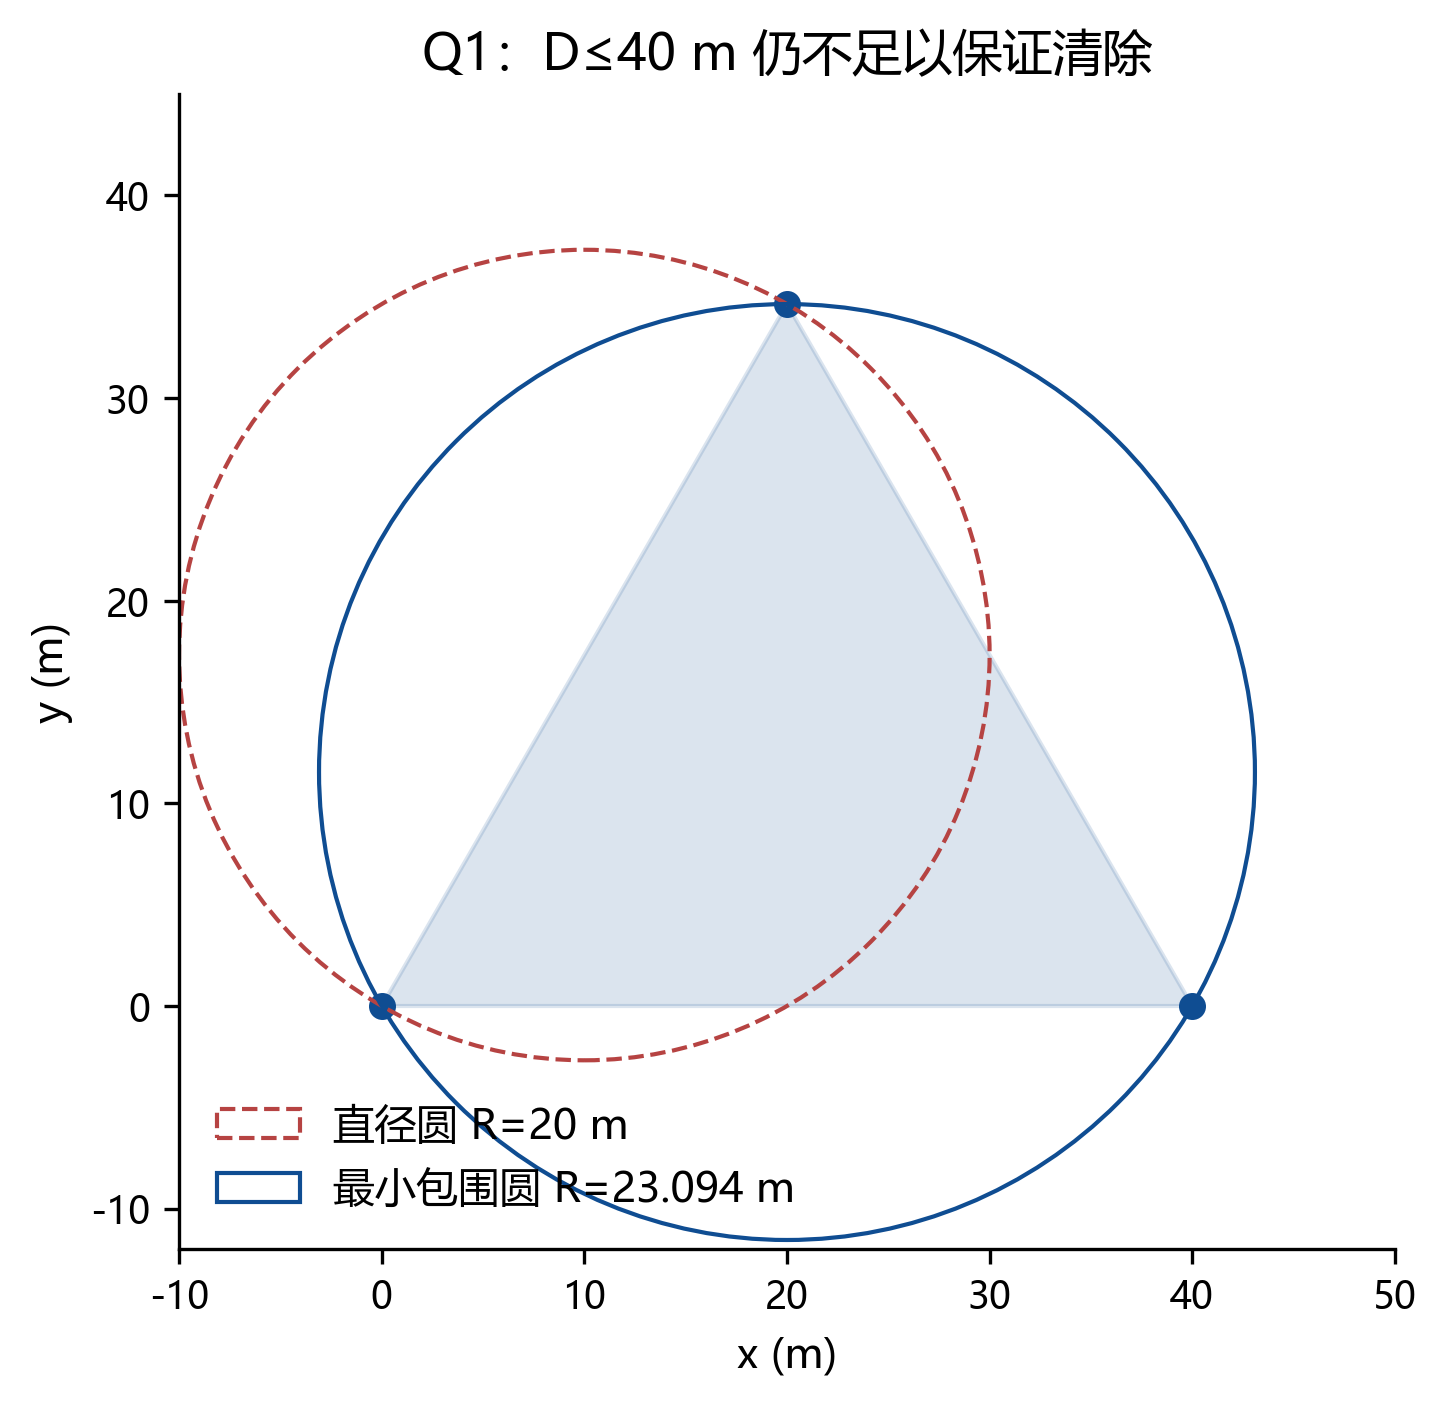
\includegraphics[width=0.64\textwidth]{figures/q1_counterexample.png}
 \caption{已有交会算例的正三角形反例。虚线直径圆不能覆盖第三个顶点；实线为最小包围圆。图与几何值来自已有结果文件，并非本轮新实验。}
 \label{fig:q1-counterexample}
\end{figure}

式\eqref{eq:q1-thales}与现有主入口的返回标记须分别理解。独立几何审计工具对输入的二进制浮点坐标转用有理数运算，枚举最远顶点对并检查该点积条件；问题一主入口中的 \texttt{diameter\_circle\_covers} 则以计算半径满足 $\widehat R\leq D/2+10^{-6}$ 作为浮点代理判断。后者不是式\eqref{eq:q1-thales}的严格实现，也不是在线清除许可。

\subsection{最小包围圆与保证清除判据}
对任意候选清除点 $c$，定义最坏位置距离
\begin{equation}
 \rho_P(c)=\max_{p\in P}\|p-c\|=\max_{v\in V(P)}\|v-c\|,
 \qquad R_{\rm MEC}(P)=\min_{c\in\mathbb R^2}\rho_P(c).
 \label{eq:q1-mec}
\end{equation}
式中的顶点表示同样由凸组合与三角不等式得到。题目规定，距离不超过 $20\,\mathrm m$ 时能够完成光学精确定位与清除，两项固定耗时分别为 $3\,\mathrm s$ 和 $2\,\mathrm s$。程序采用 $r_{\rm safe}=19.999\,\mathrm m$ 作为更保守的执行半径，其保证清除区域为
\begin{equation}
 \mathcal C_{r_{\rm safe}}(P)=\bigcap_{v\in V(P)}B(v,r_{\rm safe}),
 \qquad
 \mathcal C_{r_{\rm safe}}(P)\ne\varnothing
 \Longleftrightarrow R_{\rm MEC}(P)\leq r_{\rm safe}.
 \label{eq:q1-certificate}
\end{equation}
当实际目标属于 $P$，且提交的点 $c$ 通过所有顶点距离检查时，该点覆盖整个 $P$，从而覆盖真实目标。MEC 圆心提供这样一个候选点，但并非唯一可能的清除点。

现有包围圆函数采用增量构圆：打乱顶点顺序，依次处理落在当前圆外的点，由一个、两个或三个支持点更新圆；近共线时使用最远点对。随机增量求包围圆的算法背景见文献\cite{welzl1991}。实现固定排列种子为 $42$，并在返回前重新计算全部顶点到圆心的最大浮点距离，加上 $10^{-8}\,\mathrm m$。因此，应把输出 $\widehat R$ 与理想实数几何中的最优值 $R_{\rm MEC}$ 区分。现行执行默认仍为 MEC 圆心：计算半径不超过 $19.999\,\mathrm m$ 后，清除封装还会检查顶点及最终提交坐标；其中有理数平方距离比较针对已存储的二进制浮点坐标。该检查加强了执行点证书，但不替代对前序观测误差和区域外包正确性的要求。

\subsection{仅由直径获得的几何界与计算流程}
平面 Jung 界给出
\begin{equation}
 \frac{D(P)}2\leq R_{\rm MEC}(P)\leq\frac{D(P)}{\sqrt3}.
 \label{eq:q1-jung}
\end{equation}
左端由直径端点得到。对于右端，非退化最小包围圆或者由一对对径点确定，此时 $R=D/2$；或者由三个边界点确定且圆心位于其凸包。后一情形中，三个相邻圆心角之和为 $360^\circ$，均不超过 $180^\circ$，至少一个不小于 $120^\circ$，对应弦长至少为 $\sqrt3R$，于是 $D\geq\sqrt3R$。正三角形达到右端等号。

代入执行半径得到如下分类：
\begin{equation}
 \begin{cases}
 D(P)\leq\sqrt3r_{\rm safe}\approx34.6393\,\mathrm m:
     & \text{保证清除区域非空},\\
 \sqrt3r_{\rm safe}<D(P)\leq2r_{\rm safe}=39.998\,\mathrm m:
     & \text{直径不能决定，需进一步判定},\\
 D(P)>2r_{\rm safe}:
     & \text{不存在覆盖整个 }P\text{ 的安全清除点}.
 \end{cases}
 \label{eq:q1-thresholds}
\end{equation}
第一种情况只保证点的存在，提交前仍须构造并验证执行点；第三种情况表示当前多边形不能提供一次全覆盖证书，不表示真实目标不能被清除。若 $P$ 是外包近似，更不能由 $P$ 的不可覆盖反推真实可行集合不可覆盖。现有主流程直接计算包围圆；Jung 分类与直径圆点积检验保留在独立审计中，没有替换主流程。

\begin{table}[htbp]
 \centering\small
 \caption{问题一现有实现及独立审计的计算流程}
 \begin{tabularx}{\textwidth}{@{}c L@{}}
  \toprule
  步骤 & 操作与边界 \\
  \midrule
  1 & 读取检测点、示向度及显式误差参数，构造两个线性半平面约束。\\
  2 & 无圆域时先用线性规划判断空集、无界或坐标有界；有圆域时初始化其外包多边形。\\
  3 & 逐约束裁剪；若非空有界，调用旋转卡壳返回直径及端点，并调用增量包围圆函数。\\
  4 & 主入口返回多边形、直径、包围圆和浮点直径圆标记；独立审计另行执行式\eqref{eq:q1-thales}和\eqref{eq:q1-thresholds}。\\
  5 & 执行端采用 MEC 默认候选点；仅在半径门槛及提交点顶点距离检查均通过后，调用光学定位与清除操作。此步骤不由问题一离线入口执行。\\
  \bottomrule
 \end{tabularx}
\end{table}

\subsection{方法比较与清除判据的验证过程}
上述建模从题目给出的误差区间出发，而不是先选定一个概率分布再估计位置。若直接求两条中心示向线的交点，只能得到一个位置估计，无法表达该估计周围仍然允许存在的目标位置；若对同一地点的读数反复取平均，还会违背题目中同地点误差固定的条件。楔形交集保留了全部允许方位，因而可以将“估计点接近目标”与“任一允许目标位置均被覆盖”区分。其代价是定位区域可能偏大，需要继续移动和检测，不能由安全性优势直接推断任务耗时更短。

从计算方法看，顶点对穷举与旋转卡壳求解的是同一个多边形直径问题，前者便于核验，后者利用凸多边形的边界顺序降低计算量；从清除条件看，直径和最小包围圆回答的则是不同问题。表\ref{tab:q1-method-comparison}给出各方法的用途及适用边界。
\begin{table}[htbp]
 \centering\small
 \caption{定位与清除方法的横向比较}
 \label{tab:q1-method-comparison}
 \begin{tabularx}{\textwidth}{@{}>{\raggedright\arraybackslash}p{0.19\textwidth}L L@{}}
  \toprule
  方法 & 可提供的信息或优势 & 不能直接得到的结论或代价 \\
  \midrule
  中心示向线交点 & 给出简洁的位置估计，便于构造对照 & 不提供全部允许位置的覆盖证书 \\
  楔形交集 & 与有界误差相容，保留集合不确定性 & 外包与数值余量可能增加后续检测需求 \\
  顶点对穷举 & 直径计算易核对，复杂度为 $O(m^2)$ & 顶点较多时计算量增长较快 \\
  旋转卡壳 & 有序凸多边形的直径阶段为 $O(m)$ & 仍需处理前序求交及数值退化 \\
  仅检查 $D\leq40$ & 阈值计算简单 & 正三角形反例否定其普遍清除保证 \\
  MEC及执行点复核 & 对整个当前外包区域给出清除证书 & 未满足证书时不能据此直接清除 \\
  \bottomrule
 \end{tabularx}
\end{table}

验证过程包含数值核对与构造反例两个层次。已有几何记录保存了 $300$ 个凸多边形的直径与包围圆核对，以及 $4000$ 次目标包含检查；这些有限检查用于发现实现问题，不代替连续集合证明。图\ref{fig:q1-counterexample}的正三角形则从数学上排除了“直径不超过 $40\,\mathrm m$ 就一定能清除”的推断。后续独立审计进一步将直径圆覆盖转化为逐顶点有理数点积判据，把接近阈值时的浮点代理判断与严格几何判断分开。这样形成了从数值检查、反例检验到执行点证书的验证链条，而不是用一批未出现失败的随机样例宣称普遍正确。

相关的历史单源实验还保存了点估计与集合清除的对照。每种测点策略均包含相同的 $100$ 个源实例；将中心示向线交点作为拟清除点，以其到真实源距离是否超过 $20\,\mathrm m$ 衡量失败；集合方法则仅统计 MEC 半径不超过 $19.999\,\mathrm m$ 时的证书就绪状态。表\ref{tab:q1-stop-comparison}直接汇总已保存的距离及布尔记录，属于几何核验，不是实际清除指令日志。
\begin{table}[htbp]
 \centering\small
 \caption{历史单源算例中的点估计与集合证书对照}
 \label{tab:q1-stop-comparison}
 \begin{tabular}{@{}lrrr@{}}
  \toprule
  第二测点策略 & 点估计超出20米/实例数 & MEC就绪数 & 就绪时真实源超出20米数 \\
  \midrule
  随机安全点 & $29/100$ & 30 & 0 \\
  垂直中点 & $25/100$ & 28 & 0 \\
  NBV & $25/100$ & 23 & 0 \\
  \bottomrule
 \end{tabular}
\end{table}

点估计在 $300$ 条记录中有 $79$ 条超出清除半径，说明单点估计不足以承担保证清除的角色。MEC 就绪的 $81$ 条记录中未观察到真实源超出半径，但这只描述已就绪子集，不能写成全部 $300$ 例均已清除，也不能把不同触发次数下的失败比例当成相同代价的公平比较。该批记录中，$D\leq40$ 与 MEC 就绪标记恰好全部一致，因此它本身没有展示 MEC 相对直径阈值的经验误判率下降；两者的普遍性差异由正三角形反例和覆盖证明建立。

这一过程也揭示了安全判据与性能指标的区别：定位区域平均直径变小，未必使更多实例跨过清除半径门槛。MEC 方法的优势是将清除条件直接对应于设备的作用半径，并提供可检查的充分条件；其保守性与新增检测代价仍需在后续策略中权衡。对备选判据的比较因而同时考察保证条件、触发比例与后续动作需求，而不只比较估计误差。

\clearpage
\section{问题二：第二检测点的主动选择}
\label{sec:q2}

\subsection{首次观测区域与保证接收的候选区域}
问题二要求根据全向源的一次示向读数选择第二检测点，使交会定位获得较好的效果，并给出候选区域。题面并未强制要求第二点对所有允许目标位置均能接收信号；本文将这一条件作为保守的选点约束。记首个检测点为 $s_0$、示向度为 $\theta_0$，显式利用目标圆域及有效接收半径上界，可得连续位置集合
\begin{equation}
 \Omega_1=B(0,1800)\cap W(s_0,\theta_0,\delta)\cap B(s_0,1500).
 \label{eq:q2-prior}
\end{equation}
程序按照问题一的外包方式构造多边形 $P_1\supseteq\Omega_1$，本节数值算例使用几何函数默认误差 $\delta_{\rm impl}=1.00500001^\circ$。已获得有效示向读数还意味着距离大于 $5\,\mathrm m$，但当前多边形实现没有减去近距离圆盘；保留这部分位置使集合更保守，并保持凸性。

有效接收半径未知但至少为 $1000\,\mathrm m$，因而对全向源，可以采用
\begin{equation}
 \mathcal C_{\rm safe}(P_1)
 =\bigcap_{p\in P_1}B(p,1000)
 =\bigcap_{v\in V(P_1)}B(v,1000)
 =\left\{s:\max_{v\in V(P_1)}\|s-v\|\leq1000\right\}.
 \label{eq:q2-safe}
\end{equation}
等式由凸集顶点的距离充分性得到：若 $p=\sum_i\alpha_i v_i$，则 $\|s-p\|\leq\sum_i\alpha_i\|s-v_i\|\leq1000$。所以该区域为凸圆盘交集，对其中任意检测点和 $P_1$ 中任意目标位置，均满足最小有效接收半径约束。由于使用的是外包多边形，这只是保证接收的充分候选区域；区域外也可能接收到实际目标信号。

保证接收不等于保证返回示向度。附件规定，当距离不超过 $5\,\mathrm m$ 时返回近距离信息，可直接进入光学精确定位和清除；此时不返回方位角。本节的几何评分预测的是有示向度时的交会结果，未显式评价该近距离分支。因此，接收可行性与后验评分精度是两项不同的性质。程序按全部顶点距离不超过 $1000$ 进行浮点筛选，没有额外缩小阈值，也不将其声称为任意边界输入下的精确算术证明。

\subsection{交会几何与有限候选点}
只沿第一次示向线移动，通常不能显著增加两次观测的交会角；移向示向线侧方则可能使交会区域在两个方向同时收缩。局部线性化时，角误差对应的横向偏差随距离增大，而交会角过小会放大位置不确定性。较接近直角的交会可改善局部条件，但目标位置本身未知，长距离横移还增加耗时，故不能把 $90^\circ$ 当作独立于距离、误差与动作时间的全局最优条件。主动选择测点与权衡移动、测量成本可参考文献\cite{tokekar2011,vanderhook2014}；这些文献的观测假设及性能保证并不自动适用于本题。

以首测示向为横轴生成网格，记二维旋转矩阵为 $R(\theta_0)$，候选集合写为
\begin{equation}
 \begin{split}
 \mathcal S_{\rm grid}=
 \{s_0+R(\theta_0)(a,b)^{\mathsf T}:\ &a=0,50,\ldots,1500,\\[-2pt]
                                      &b=-600,-560,\ldots,600\},\\
 \mathcal S=\mathcal S_{\rm grid}\cap\mathcal C_{\rm safe}(P_1).
 \end{split}
 \label{eq:q2-grid}
\end{equation}
该式是现有 $s_0=(0,0)$ 算例的坐标表达，原入口固定首测点为原点、首测示向度为 $30^\circ$，不应据此声称已实现任意首测输入的通用命令接口。原始网格共有 $31\times31=961$ 个点，已有结果保留 $213$ 个安全候选点。有限网格仅用于数值搜索，不等同于连续候选区域本身。通用选点辅助函数还提供围绕几何中心与长轴生成候选点的方式，但本例显式传入上述网格，没有使用该默认候选生成器。

\subsection{采样后验直径与动作时间评分}
对于候选点 $s$，理想的稳健评价需考虑 $P_1$ 内所有目标位置及全部允许测向误差，计算第二次观测后定位直径的最大值。当前实现用有限情景近似该问题。先取多边形顶点及顶点坐标的算术均值作为位置代表；若代表数超过 $9$，按数组索引等距抽取 $9$ 个。这里的算术均值不是多边形面积质心，也不是目标位置的概率期望。将代表集合记为 $\mathcal G$，误差代表为
\begin{equation}
 \mathcal E=\{-\delta_{\rm impl},0,\delta_{\rm impl}\}.
\end{equation}
令 $\operatorname{atan2}_{\deg}=(180/\pi)\operatorname{atan2}$ 表示以度为单位的方位角。对每个 $(g,e)\in\mathcal G\times\mathcal E$，构造预测示向度
$\widehat\theta(s;g,e)=\operatorname{atan2}_{\deg}(g_y-s_y,g_x-s_x)+e$，并定义
\begin{equation}
 \begin{split}
 P_2(s;g,e)&=P_1\cap W(s,\widehat\theta(s;g,e),\delta_{\rm impl}),\\
 \widehat D_{\rm worst}(s)&=
 \max_{\substack{g\in\mathcal G,\ e\in\mathcal E\\P_2(s;g,e)\ne\varnothing}}
 D\bigl(P_2(s;g,e)\bigr).
 \end{split}
 \label{eq:q2-sampled}
\end{equation}
这里的“最坏”仅指已采样情景中的最大值。取多边形顶点足以计算固定圆心的最远距离，但不意味着顶点及三种误差足以实现非线性的连续最坏后验搜索。本例 $P_1$ 有 $4$ 个顶点，加上顶点均值共 $5$ 个位置代表，故每个候选点评价 $15$ 个预测示向情景。已有候选记录中，各候选距首测点至少为 $550\,\mathrm m$，因此本例没有同点重测。当前预测只叠加楔形，没有再次加入 $1500\,\mathrm m$ 接收距离圆、近距离返回分支或同地点固定误差的历史约束。

机器狗速度为 $5\,\mathrm{m/s}$，一次测向的固定时间为 $5\,\mathrm s$。在延续首测目标频道的条件下，不需要换频，第二次测向的新增动作时间及评分为
\begin{equation}
 T(s)=\frac{\|s-s_0\|}{5\,\mathrm{m/s}}+5\,\mathrm s,
 \qquad
 J_\lambda(s)=\widehat D_{\rm worst}(s)+\lambda T(s),
 \quad [\lambda]=\mathrm{m/s}.
 \label{eq:q2-objective}
\end{equation}
由此选择
\begin{equation}
 s_1\in\operatorname*{arg\,min}_{s\in\mathcal S}J_\lambda(s).
 \label{eq:q2-choice}
\end{equation}
该评分把定位尺度与动作耗时统一为长度量纲。$\lambda=0$ 只比较采样定位直径；增大 $\lambda$ 会提高移动和测量时间的相对权重。首测已经发生的耗时不计入此次增量，后续清除时间也不包含在本评分中。若切换频道，题目规定另加 $1\,\mathrm s$，但问题二同频道算例没有这项操作。式\eqref{eq:q2-choice}是有限候选集合上的枚举最小值，不是连续检测平面上的全局鲁棒最优解。

通用辅助函数允许保留不安全候选点，并把未接收信号时的后验直径保守地取为原直径 $D(P_1)$。问题二入口实际设置 \texttt{safe\_only=True}，因而在评分前即剔除了这类候选，未使用该无信号分支。若安全网格为空，现有辅助函数报告没有可用候选；这只能说明当前离散搜索失败，不能证明连续安全候选区域为空。

\subsection{已有数值算例及适用边界}
取已有算例中的 $s_0=(0,0)$、$\theta_0=30^\circ$，保持候选点与所有后验评分不变，仅改变 $\lambda$，所得结果如表\ref{tab:q2-results}。数值直接取自现有 \texttt{q2.json} 及候选记录 \texttt{q2\_candidates.csv}，本轮没有重新运行求解或模拟器。

\begin{table}[htbp]
 \centering
 \caption{同一离散算例在不同时间权重下的选点结果}
 \label{tab:q2-results}
 \begin{tabular}{@{}rrrrr@{}}
  \toprule
  $\lambda\ (\mathrm{m/s})$ & $x\ (\mathrm m)$ & $y\ (\mathrm m)$ & $\widehat D_{\rm worst}\ (\mathrm m)$ & $T\ (\mathrm s)$ \\
  \midrule
  0   & 476.12 & 875.33 & 112.92 & 204.29 \\
  0.2 & 476.12 & 875.33 & 112.92 & 204.29 \\
  1   & 326.22 & 834.97 & 130.45 & 184.29 \\
  5   & 336.31 & 517.49 & 241.87 & 128.43 \\
  \bottomrule
 \end{tabular}
\end{table}

在该有限候选集上，$\lambda=0$ 与 $0.2$ 选择同一点；增大至 $1$ 时，以更大的采样后验直径换取较短的新增动作时间；$\lambda=5$ 进一步偏向距离首测点较近的位置。图\ref{fig:q2-candidates}展示已保留的 $213$ 个候选点及其采样评分。图中的点云是离散筛选结果，并非对连续区域边界的完整刻画。上述结果说明本例中的定位质量与移动时间存在权衡，不能用来证明某一权重对其他初始观测或整局任务具有普遍最优性。

\begin{figure}[H]
 \centering
 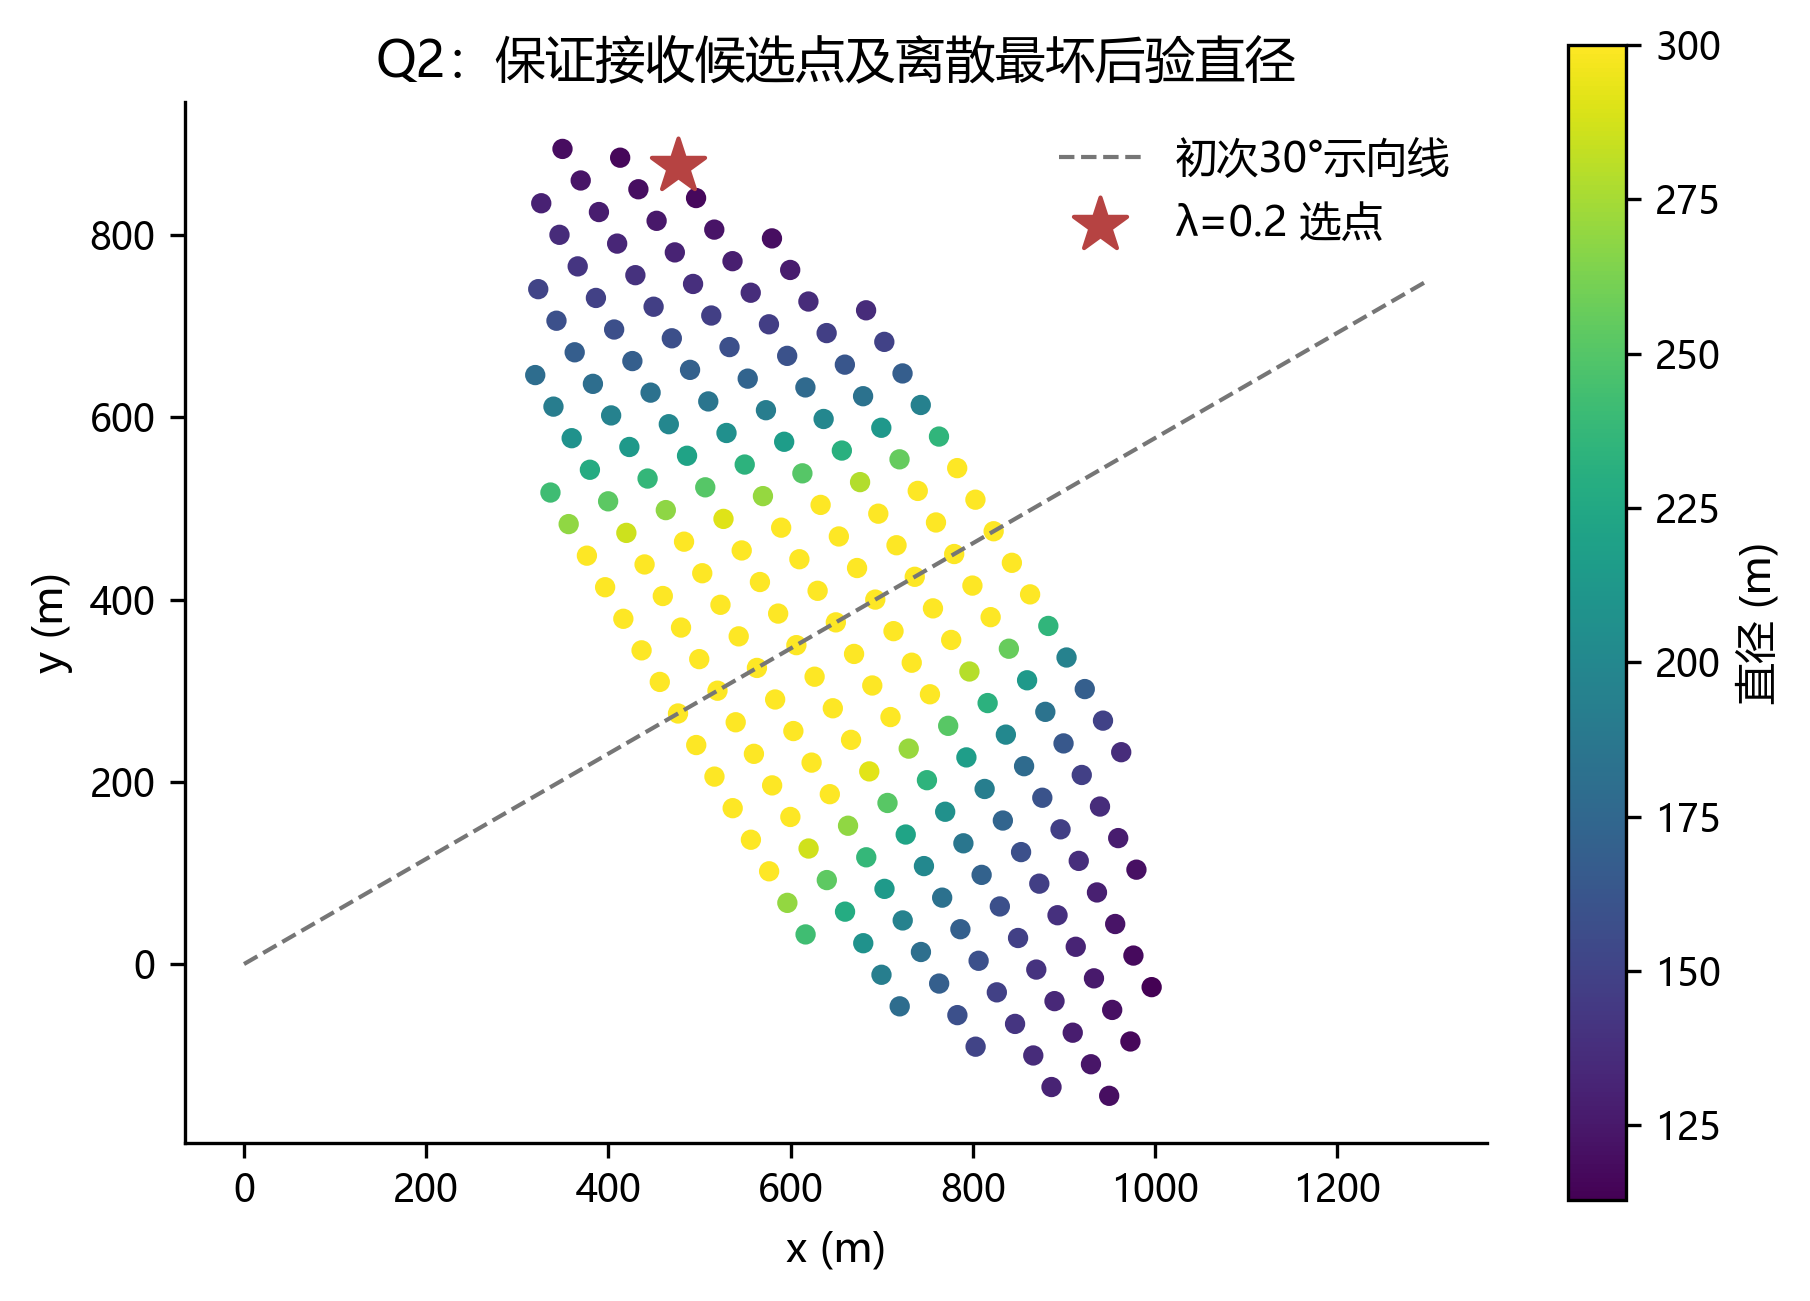
\includegraphics[width=0.78\textwidth]{figures/q2_candidates.png}
 \caption{首测示向度 $30^\circ$ 的已有安全候选点。颜色表示采样情景中的最大后验直径，星号为 $\lambda=0.2\,\mathrm{m/s}$ 的选点；颜色显示上限为 $300\,\mathrm m$，更大数值采用上限颜色。}
 \label{fig:q2-candidates}
\end{figure}

\begin{table}[H]
 \centering\small
 \caption{问题二现有离散选点流程}
 \begin{tabularx}{\textwidth}{@{}c L@{}}
  \toprule
  步骤 & 操作 \\
  \midrule
  1 & 构造首测楔形与圆约束的外包多边形 $P_1$，建立旋转网格。\\
  2 & 对每个候选点计算其到全部顶点的最大距离，保留不超过 $1000\,\mathrm m$ 的点。\\
  3 & 取顶点及顶点均值，必要时压缩至 $9$ 个代表；分别施加三种误差，裁剪预测楔形并计算后验直径。\\
  4 & 汇总每点的最大采样后验直径与移动加测向时间，枚举最小化式\eqref{eq:q2-objective}。\\
  5 & 输出选点、候选记录及采样评分。问题二入口到此结束，不调用检测或清除接口。\\
  \bottomrule
 \end{tabularx}
\end{table}

\subsection{备选策略对比与时间权衡的形成}
第二测点策略的比较从随机安全点、交会角启发式和主动选点三个层次展开。随机安全点不主动优化后验形状；垂直中点法依据首测区域的暂定中心，在首测示向线侧方布置检测点，以改善交会角；NBV 则对有限预测观测计算后验直径，并加入移动与检测时间。垂直中点是针对未知源位置的几何启发式，不是利用真实源位置构造的理想 $90^\circ$ 测点。三种方法的共同出发点是首测集合，差异在于如何使用该集合决定下一次观测。

已有的历史单源消融为每种策略保存了 $100$ 个同种子实例，源有效半径统一设为 $1500\,\mathrm m$，其结果见表\ref{tab:q2-historical}。这组实验使用通用候选生成器，NBV 没有启用本节 $213$ 点算例的强制安全筛选，只有随机安全点明确从安全候选中抽取。故该表可比较三种既有策略在相同源实例下的表现，不能把差异全部归因于评分公式这一项改变。表中时间包含第一次与第二次检测，亦不同于表\ref{tab:q2-results}仅计第二动作新增时间的口径。
\begin{table}[htbp]
 \centering
 \caption{历史100个单源算例的第二测点策略比较}
 \label{tab:q2-historical}
 \begin{tabular}{@{}lrrr@{}}
  \toprule
  策略 & 实例数 & 平均后验直径/米 & 前两次检测平均累计时间/秒 \\
  \midrule
  随机安全点 & 100 & 136.62 & 162.99 \\
  垂直中点 & 100 & 76.21 & 165.30 \\
  NBV & 100 & 72.17 & 188.32 \\
  \bottomrule
 \end{tabular}
\end{table}

相对随机安全点，NBV 的平均后验直径减少约 $47.18\%$，但平均时间增加约 $15.54\%$；相对垂直中点，平均直径减少约 $5.31\%$，平均时间增加约 $13.92\%$。逐种子比较中，NBV 相对随机安全点在直径上有 $53$ 例改善、$13$ 例相同、$34$ 例变差；相对垂直中点则为 $52$ 例改善、$48$ 例变差，且 $100$ 例均耗时更长。这表明平均直径优势不是逐例优势，更不是时间与定位质量的同时占优。

\begin{figure}[H]
 \centering
 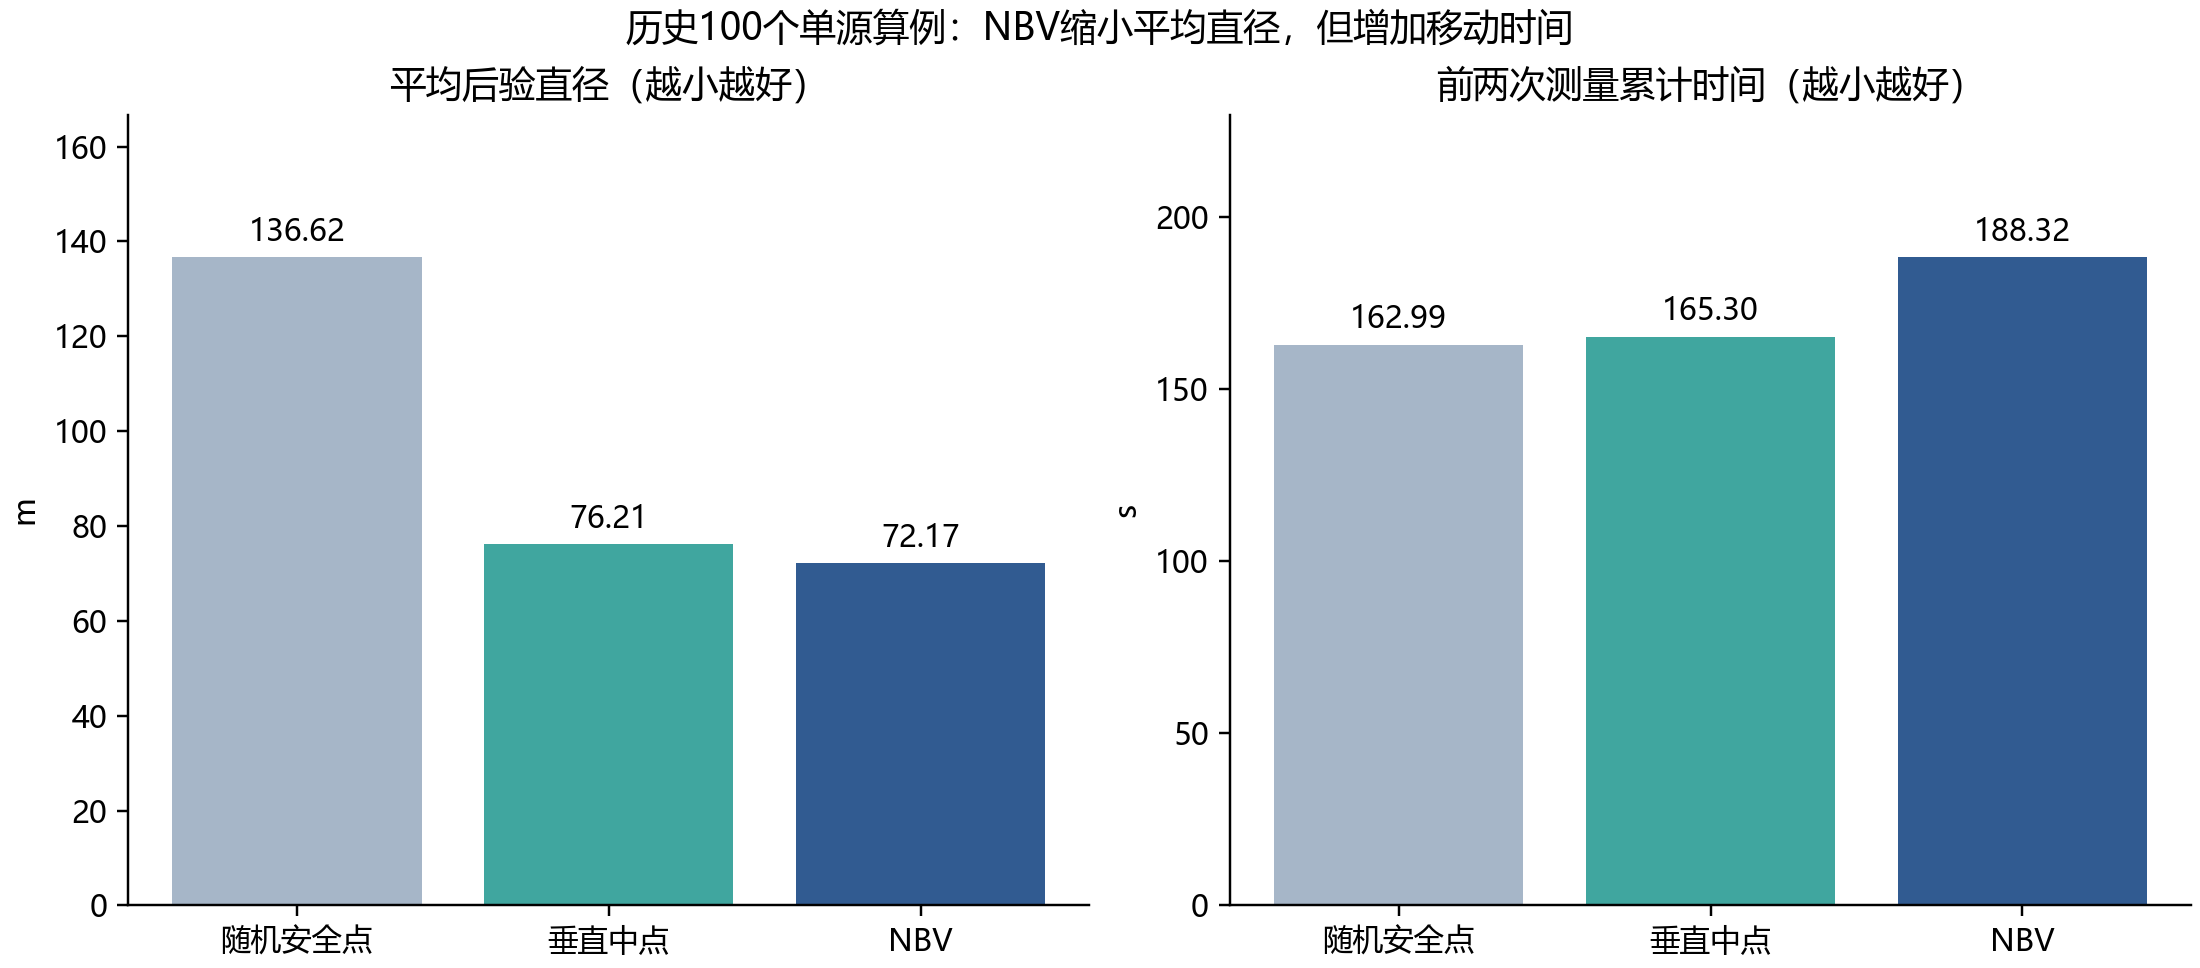
\includegraphics[width=0.98\textwidth]{figures/q2_historical_tradeoff.png}
 \caption{历史单源策略的定位尺度与时间代价。图由保存的300条记录重新汇总绘制，未新增模拟实验；两个纵轴分别使用米与秒，均从零开始。}
 \label{fig:q2-historical-tradeoff}
\end{figure}

由此需要进一步区分三类改进。首先，安全候选区域解决“是否能够收到信号”，这是相对无约束启发式的可行性加强，但会限制可选站位。其次，采样后验评分解决“哪些有限观测情景可能使定位区域收缩”，它在历史算例中降低了平均直径，却不保证每例都更好。最后，时间项显式暴露了几何收缩所付出的移动代价；固定 $213$ 个候选及其情景评分，再仅改变 $\lambda$，可得到表\ref{tab:q2-results}所示的可复核权重比较，而不会把候选生成器变化与时间权重变化混在一起。

在该固定候选算例中，将 $\lambda$ 从 $0.2$ 提高到 $1$，第二动作时间由 $204.29\,\mathrm s$ 降至 $184.29\,\mathrm s$，同时最大采样后验直径由 $112.92\,\mathrm m$ 增至 $130.45\,\mathrm m$；继续增大权重会进一步偏向短距离站位。该结果支持将时间作为可调决策偏好，而不支持宣称时间权重必然同时改善两个指标。上述验证将候选可行性、定位尺度与动作时间分开比较，使每项结论具有对应的证据和适用范围。

与问题一的清除证书对应，表\ref{tab:q1-stop-comparison}还显示，NBV 虽具有最小的平均后验直径，其第二次观测后的 MEC 就绪数却不是最多。这说明最小化平均定位尺度和尽快达到清除门槛并非等价目标；仅凭均值不能推断整局清除效率。当前方法保留“集合约束确保允许位置不被主动排除、证书控制清除、时间评分选择观测”的分工。其已有优势在于与有界误差和实际动作成本相容、每一决策量可复核；尚未得到连续最坏情景误差界或整局时间最优保证，面向后续清除时间的多步优化也不作为已经实现的收益。

\clearpage
\bibliographystyle{gbt7714-numerical}
\bibliography{references}
\end{document}
